\documentclass[conference]{IEEEtran}
\IEEEoverridecommandlockouts
\usepackage{cite}
\usepackage{amsmath,amssymb,amsfonts}
\usepackage{mathtools}
\usepackage{algorithmic}
\usepackage{graphicx}
\usepackage{textcomp}
\usepackage{xcolor}
\usepackage{booktabs}
\usepackage{multirow}
\usepackage{url}

\def\BibTeX{{\rm B\kern-.05em{\sc i\kern-.025em b}\kern-.08em
    T\kern-.1667em\lower.7ex\hbox{E}\kern-.125emX}}

\begin{document}

\title{MonoArm: A Reproducible Benchmarking Framework for Monocular\\
Upper-Limb Joint Angle Estimation, with Real-Data Validation\\
on CMU Panoptic Studio}

\author{
\IEEEauthorblockN{Author Name Withheld for Draft}
\IEEEauthorblockA{\textit{Department (to be completed)} \\
\textit{Institution (to be completed)} \\
City, Country \\
email@domain.example}
}

\maketitle

\begin{abstract}
Monocular RGB pose estimation is an attractive low-cost alternative to
marker-based motion capture for rehabilitation robotics, exoskeleton
calibration, and human--computer interaction, but published systems are
rarely evaluated against 3D ground truth with the statistical rigor
expected of a measurement instrument. We present MonoArm, a reproducible
benchmarking framework that computes anatomically consistent bilateral
shoulder and elbow joint angles from three 2D pose estimators (MediaPipe
BlazePose, MoveNet, and PoseNet) using a torso-relative coordinate frame
and a ZXY Euler decomposition, ablates three causal temporal filters
(moving average, Savitzky--Golay, and a two-state Kalman filter) against
ground truth rather than against the unfiltered signal alone, and applies
a full statistical-significance protocol (paired $t$-test, Wilcoxon
signed-rank test, Cohen's $d_z$, bootstrap confidence intervals, and
Holm--Bonferroni correction) to framework comparisons. Because access to
Human3.6M is registration-gated and was unavailable during this study, we
validate the framework instead on a real, non-simulated sequence from the
publicly distributed CMU Panoptic Studio dataset, running the actual pose
estimators on real video and scoring them against real 3D motion-capture
ground truth end to end. A first pass of this validation assumed video
frame $i$ and ground-truth frame $i$ referred to the same instant; a
correlation-based check on a wraparound- and reliability-gate-free
reference channel revealed this assumption was wrong by a consistent
$\sim\!10$ frames, and we report a procedure -- fixed in advance on a
single reference framework and channel, not tuned per result -- for
detecting and correcting this class of error, which we believe is an
underappreciated hazard whenever separately-captured video and
motion-capture streams are paired by filename index rather than verified
timestamp. After correction (91 of the original 101 frames retain a
valid pairing), MoveNet-Lightning achieved a lower mean per-joint angle
error (26.7\textdegree\ vs.\ 44.8\textdegree) and higher correlation with
ground truth ($r=0.789$ vs.\ $r=0.669$) than MediaPipe on this pilot
sequence. In further diagnosing these results we identify two additional
evaluation pitfalls that would otherwise bias any framework comparison
built on Euler-angle joint parameterizations: (i) naive degree-wise
differencing overstates flexion error by 12--35\% whenever the true
angle path crosses the $\pm180^\circ$ discontinuity of an
\texttt{atan2}-based decomposition, and (ii) treating a
geometrically-unobservable rotation estimate as a valid measurement
produces framework-dependent, oppositely-signed bias. We report raw,
wraparound-corrected, and reliability-conditioned metrics throughout,
quantify the mechanism behind each pitfall, and discuss the framework's
remaining limitations -- including the small, single-subject scale of
the real-data pilot, and the fact that repeated-measures significance
testing on one continuous motion sequence should be read descriptively
rather than as a properly powered inferential result.
\end{abstract}

\begin{IEEEkeywords}
monocular pose estimation, joint angle estimation, MediaPipe, MoveNet,
PoseNet, human motion capture, benchmarking, Kalman filter, Human3.6M,
CMU Panoptic Studio
\end{IEEEkeywords}

\section{Introduction}

Restoring and assisting human arm movement is a central goal of
rehabilitation robotics and wearable assistive technology. Soft wearable
exoskeletons are increasingly proposed as low-cost, comfortable
alternatives to rigid assistive devices, but their calibration and
validation still typically require marker-based motion capture --
expensive, lab-bound, and impractical for continuous use outside a
research setting. Monocular RGB pose estimation offers a non-contact
alternative: a single camera and a 2D keypoint detector can, in
principle, supply the joint-angle reference signal that such systems
need, at a fraction of the cost.

The practical obstacle is trust. A system intended as a calibration or
validation reference must itself be validated, and the majority of
monocular arm-tracking demonstrations in the literature and in student
projects report qualitative smoothness (``the avatar's arm moves like
mine'') rather than quantitative agreement with 3D ground truth,
statistical tests of framework differences, or an explicit accounting of
where the underlying angle mathematics can fail. This is understandable:
the standard ground-truth resource for this kind of validation, Human3.6M
(H3.6M) \cite{ionescu2014human36m}, requires researcher registration at
\url{vision.imar.ro}, and that registration process has been effectively
closed to new applicants for an extended period at the time of this
work, leaving many groups without a path to real quantitative validation
at all.

This paper makes four contributions. First, we describe MonoArm, a
benchmarking framework that computes four anatomically consistent
bilateral joint angles (shoulder flexion-extension, shoulder
abduction-adduction, shoulder internal-external rotation, and elbow
flexion) from three widely used 2D pose estimators under a common
coordinate convention, so that framework, filter, and dataset can be
varied independently. Second, in place of the registration-gated H3.6M,
we validate the framework end to end -- real pose estimators, on real
video, scored against real 3D motion-capture ground truth -- using a
publicly distributed sequence from the CMU Panoptic Studio dataset
\cite{joo2015panoptic}, and report the resulting comparison between
MediaPipe and MoveNet-Lightning (PoseNet could not be evaluated in our
deployment environment for a documented, reproducible reason given in
Section~\ref{sec:setup}). Third, we report a concrete case in which the
naive assumption that a video stream and a separately-reconstructed
motion-capture stream share a common frame index was wrong by a
consistent margin, and give a pre-registered, non-circular procedure for
detecting and correcting this -- a step we believe should be standard
practice whenever such streams are paired by filename rather than
verified timestamp, and one that materially changed our own reported
numbers. Fourth, having corrected for that, we identify and quantify two
further evaluation pitfalls -- an angle-wraparound artifact and a
rotation-observability confound -- that inflate or bias error metrics in
ways specific to Euler-angle parameterizations of joint orientation, and
that we believe generalize to other monocular joint-angle benchmarking
efforts using a similar decomposition.

We emphasize at the outset that the real-data validation presented here
is a single-subject, single-camera pilot of 101 raw frames (91 after the
temporal-alignment correction of Section~\ref{sec:sync}), not a
large-\textit{N} benchmark; Section~\ref{sec:limitations} discusses this
scope limitation and what a full H3.6M-scale validation under the same
framework would add.

\section{Related Work}

\subsection{Monocular 2D Pose Estimation}
MediaPipe Pose is built on BlazePose \cite{bazarevsky2020blazepose}, a
lightweight two-stage (detector + regressor) convolutional network that
predicts 33 pseudo-3D landmarks and is optimized for real-time mobile
inference. MoveNet \cite{movenet2021blog} is a single-shot
center-tracking architecture released by Google in Lightning
(latency-optimized) and Thunder (accuracy-optimized) variants; unlike the
other two frameworks studied here, MoveNet was announced through
TensorFlow's engineering blog rather than a peer-reviewed publication, so
we cite the primary technical source available. PoseNet, as used in this
study, is the TensorFlow Lite MobileNetV1 heatmap-and-offset decoder
whose bottom-up, part-based grouping approach traces to PersonLab
\cite{papandreou2018personlab}.

\subsection{Anatomical Angle Extraction and Filtering}
Extracting clinically meaningful joint angles from 2D or pseudo-3D
keypoints requires a body-relative reference frame; we follow the
International Society of Biomechanics (ISB) recommendation for the
shoulder, elbow, wrist, and hand \cite{wu2005isb}, adapted to a ZXY
Euler sequence for numerical reasons discussed in
Section~\ref{sec:angles}, and draw on prior reconstructions of arm
kinematics from spatial tracking data \cite{biryukova2000kinematics} for
the two-link rigid-segment model. Real-time smoothing of noisy angle
estimates is a classical signal-processing problem; we compare a
two-state Kalman filter \cite{kalman1960new} against Savitzky--Golay
polynomial smoothing \cite{savitzky1964smoothing} and a plain moving
average.

\subsection{Benchmark Datasets}
Human3.6M \cite{ionescu2014human36m} is the de facto standard for 3D
human pose evaluation, providing 3.6 million frames of synchronized video
and MoCap-derived 3D joint positions for seven subjects performing
scripted actions, but access requires an approved researcher account.
CMU Panoptic Studio \cite{joo2015panoptic} is a 480-camera dome capture
system built for markerless social-interaction motion capture; a subset
of its sequences, including 3D body keypoints reconstructed from the
dome's HD cameras, is distributed without a registration gate and has
been used elsewhere as a substitute validation source when H3.6M is
unavailable. We use it in that role here.

\subsection{Evaluation Methodology}
Mean Per-Joint Position/Angle Error and Percentage of Correct Keypoints
(PCK) are standard in the pose estimation literature
\cite{yang2011articulated,mehta2017vnect}; we adopt the angular analogue,
Mean Per-Joint Angle Error (MPJAE), following the convention used for
monocular 3D pose validation in VNect \cite{mehta2017vnect}. For
determining whether differences between frameworks are statistically
meaningful rather than incidental, we use paired significance testing
(Wilcoxon signed-rank \cite{wilcoxon1945individual}), effect-size
reporting (Cohen's $d_z$ \cite{cohen1988statistical}), and
multiple-comparison correction (Holm--Bonferroni
\cite{holm1979simple}); Bland--Altman analysis \cite{bland1986statistical}
supplements correlation-based agreement plots, which are known to be
insufficient on their own for assessing measurement agreement.

\section{System Architecture and Methodology}

\subsection{Pipeline Overview}
MonoArm processes each video frame through a common
\texttt{PoseEstimator} interface implemented independently for
MediaPipe, MoveNet (Lightning/Thunder), and PoseNet, so that the
framework identity is a single swappable factor in the evaluation. Each
estimator returns a 33-point MediaPipe-convention landmark list (COCO-17
outputs from MoveNet/PoseNet are remapped onto it). From this landmark
list, a torso-relative coordinate frame is constructed once per frame and
shared by both arms; four joint angles per arm are then computed from it;
and, in the ablation stage only, one of three causal temporal filters is
applied. Raw (unfiltered) predictions are what is scored against ground
truth for framework comparison, so that framework accuracy and filter
effect are never conflated -- filtering is evaluated as a separate,
explicit factor (Section~\ref{sec:filtering}).

\subsection{Torso Coordinate Frame}
Camera-space landmark coordinates are not directly interpretable as
anatomical angles: the same physical shoulder pose produces different
raw coordinates depending on camera tilt and the subject's stance. We
therefore construct an orthonormal torso frame from the four torso
landmarks (left/right shoulder, left/right hip) once per frame. Writing
$\mathbf{h}_{mid}$ and $\mathbf{s}_{mid}$ for the hip and shoulder
midpoints,
\begin{align}
\hat{\mathbf{y}} &= \operatorname{norm}(\mathbf{s}_{mid} - \mathbf{h}_{mid}) &&\text{(superior)}\\
\mathbf{x}_{c} &= \operatorname{norm}(\mathbf{s}_{L} - \mathbf{s}_{R}) &&\text{(lateral candidate)}
\end{align}
Because noisy keypoints make $\mathbf{x}_c$ and $\hat{\mathbf{y}}$ only
approximately orthogonal, one step of Gram--Schmidt orthogonalization is
applied:
\begin{align}
\mathbf{x}' &= \mathbf{x}_c - (\mathbf{x}_c\cdot\hat{\mathbf{y}})\hat{\mathbf{y}}, &
\hat{\mathbf{z}} &= \operatorname{norm}(\mathbf{x}' \times \hat{\mathbf{y}}) \\
\hat{\mathbf{x}} &= \operatorname{norm}(\hat{\mathbf{y}} \times \hat{\mathbf{z}}) &&
\end{align}
giving a right-handed frame $R = [\hat{\mathbf{x}}\;\hat{\mathbf{y}}\;\hat{\mathbf{z}}]$
with $\hat{\mathbf{x}}$ lateral (toward the subject's left),
$\hat{\mathbf{y}}$ superior, and $\hat{\mathbf{z}}$ anterior. A world
vector is expressed in torso coordinates as $\mathbf{v}_{torso} =
R^{\!\top}\mathbf{v}_{world}$.

\subsection{Shoulder and Elbow Angle Decomposition}
\label{sec:angles}
Let $\mathbf{v} = (v_x, v_y, v_z)$ be the unit upper-arm vector
(shoulder$\to$elbow) in torso coordinates. We decompose shoulder
orientation with a ZXY Euler sequence rather than the ISB-recommended
YXY sequence, because YXY is singular exactly at the arm-hanging rest
pose ($\mathbf{v}\approx(0,-1,0)$), the most frequently occupied pose in
natural motion; ZXY relocates the singularity to the arm pointing
directly at the camera, which is rare in practice, but -- as
Section~\ref{sec:results} shows -- it introduces a second, less obvious
singularity at full abduction. Flexion-extension and
abduction-adduction are
\begin{align}
\theta_{flex} &= \operatorname{atan2}(-v_z, -v_y) \\
\theta_{abd} &= \arcsin(\operatorname{clip}(-v_x, -1, 1))
\end{align}
(the sign convention on $v_x$ accounts for $\hat{\mathbf{x}}$ pointing to
the subject's left while the angle reported is for the right arm; the
left arm is handled by the reflection in Section~\ref{sec:bilateral}).
Elbow flexion, from the forearm unit vector $\hat{\mathbf{f}}$
(elbow$\to$wrist) and upper-arm unit vector $\hat{\mathbf{u}}$ (both
proximal$\to$distal), is
\begin{equation}
\theta_{elbow} = \arccos(\operatorname{clip}(\hat{\mathbf{u}}\cdot\hat{\mathbf{f}}, -1, 1)),
\end{equation}
giving $0^\circ$ for a fully extended arm and $\sim\!150^\circ$ at
maximal flexion.

Shoulder internal/external rotation cannot be recovered from the
upper-arm vector alone -- axial spin of the humerus does not move the
elbow. We use the forearm as a proxy, projecting it onto the plane
perpendicular to the upper-arm axis:
\begin{equation}
\mathbf{f}_\perp = \hat{\mathbf{f}} - (\hat{\mathbf{f}}\cdot\hat{\mathbf{u}})\hat{\mathbf{u}}, \qquad
\theta_{rot} = \operatorname{atan2}(\mathbf{f}_\perp\!\cdot\!\mathbf{e}_1,\ \mathbf{f}_\perp\!\cdot\!\mathbf{e}_2)
\end{equation}
for an orthonormal basis $(\mathbf{e}_1, \mathbf{e}_2)$ of that plane.
This projection is only well-conditioned when the elbow is bent enough
that $\|\mathbf{f}_\perp\|$ is bounded away from zero; MonoArm gates the
estimate as unreliable below $25^\circ$ of elbow flexion and reports a
placeholder value with a reliability flag rather than a noise-dominated
angle. As Section~\ref{sec:results} shows, whether an evaluation
pipeline respects this flag materially changes the measured rotation
error.

\subsection{Bilateral Symmetry}
\label{sec:bilateral}
Rather than duplicating the above formulas with flipped signs for the
left arm, MonoArm reflects the left arm's torso-frame vectors across the
sagittal plane, $(v_x,v_y,v_z)\mapsto(-v_x,v_y,v_z)$, before applying the
right-arm formulas unchanged. A reflected left arm is geometrically
indistinguishable from a right arm, so the same equations yield
anatomically mirrored conventions (abduction positive $=$ away from the
midline, internal rotation positive, for both arms) without a second
code path. Elbow flexion needs no reflection, since a dot product is
reflection-invariant. The same reflection is applied identically in the
ground-truth extractors for both H3.6M and CMU Panoptic
(Section~\ref{sec:setup}), so predictions and ground truth are always
compared in the same angle space.

\subsection{Temporal Filtering}
\label{sec:filtering}
Three causal filters are implemented per angle channel. The moving
average, $y[n]=\frac1W\sum_{k=0}^{W-1}x[n-k]$, is a cheap baseline with
$(W\!-\!1)/2$ frames of group delay. Savitzky--Golay
\cite{savitzky1964smoothing} fits a degree-$p$ polynomial to a window
and evaluates it at the most recent sample, preserving curvature and
peak timing better than a flat mean. The two-state Kalman filter models
state $\mathbf{x}=[\theta,\dot\theta]^{\!\top}$ under a constant-velocity
transition $F=\begin{bsmallmatrix}1&dt\\0&1\end{bsmallmatrix}$ with
measurement matrix $H=[1\ 0]$, discretized white-noise-acceleration
process covariance
$Q = q\begin{bsmallmatrix}dt^4/4 & dt^3/2\\ dt^3/2 & dt^2\end{bsmallmatrix}$,
and the standard predict/update recursion
\begin{align}
\mathbf{x}^- &= F\mathbf{x}, & P^- &= FPF^{\!\top}+Q \\
K &= P^-H^{\!\top}(HP^-H^{\!\top}+R)^{-1} \\
\mathbf{x} &= \mathbf{x}^- + K(z-H\mathbf{x}^-), & P &= (I-KH)P^-.
\end{align}
Because the state includes angular velocity, the predict step
extrapolates through fast motion, reducing the lag that afflicts the
moving average and, to a lesser extent, Savitzky--Golay. Filtering is
applied identically per angle channel and reset at sequence boundaries
so it never smooths across a subject or action transition; it is
evaluated as an explicit ablation factor (none / MA / SG / Kalman)
against ground truth, not merely against the unfiltered signal, so that
filters can be compared on accuracy and jitter reduction rather than
smoothness alone.

\subsection{Evaluation Metrics and Statistical Protocol}
\label{sec:metrics}
For predicted/ground-truth angle pairs $\{(p_i, g_i)\}_{i=1}^{N}$ (frames
with either signal missing are excluded, never imputed), we report Mean
Absolute Error (MAE), Root Mean Squared Error (RMSE), signed bias
$\frac1N\sum(p_i-g_i)$, Pearson correlation $r$, coefficient of
determination $R^2$, Percentage of Correct Keypoints at
$5^\circ/10^\circ/15^\circ$ (PCK@$\theta$: fraction of frames with
$|p_i-g_i|<\theta$), and jitter (mean $|\Delta p|$ frame-to-frame, a
stability proxy). MPJAE is the macro-average of MAE across the four
joint DOF. For comparing two frameworks on the same frames we use a
paired $t$-test and, as a distribution-free alternative given the
heavy-tailed nature of pose error, the Wilcoxon signed-rank test on the
per-frame absolute-error differences, report Cohen's $d_z$ as an effect
size, compute percentile bootstrap confidence intervals, and apply
Holm--Bonferroni correction across the resulting family of tests.

\section{Experimental Setup}
\label{sec:setup}

\subsection{Ground Truth Source}
Human3.6M \cite{ionescu2014human36m} registration at
\url{vision.imar.ro} was unavailable throughout this study. We therefore
validate the live pipeline on a publicly distributed CMU Panoptic Studio
\cite{joo2015panoptic} sequence (\texttt{171204\_pose1\_sample}), which
provides synchronized HD video and per-frame 3D body keypoints
(``coco19'' skeleton) reconstructed from the dome's calibrated camera
array -- a genuine, non-registration-gated 3D motion-capture ground
truth. Right-arm bilateral ground-truth angles are computed from the
\texttt{rShoulder}/\texttt{rElbow}/\texttt{rWrist} coco19 joints using
the identical torso-frame construction and ZXY decomposition described
in Section~\ref{sec:angles}, so predictions and ground truth share one
angle convention. We use HD camera \texttt{00\_00} and all 101 frames
(3.4~s at 29.97~fps) for which both a 3D reconstruction and a video frame
exist. Fig.~\ref{fig:sample} shows a representative frame; the subject
is a Panoptic Studio capture participant included in the dataset's
public research release, not a participant recruited for this study.

\begin{figure}[t]
\centering
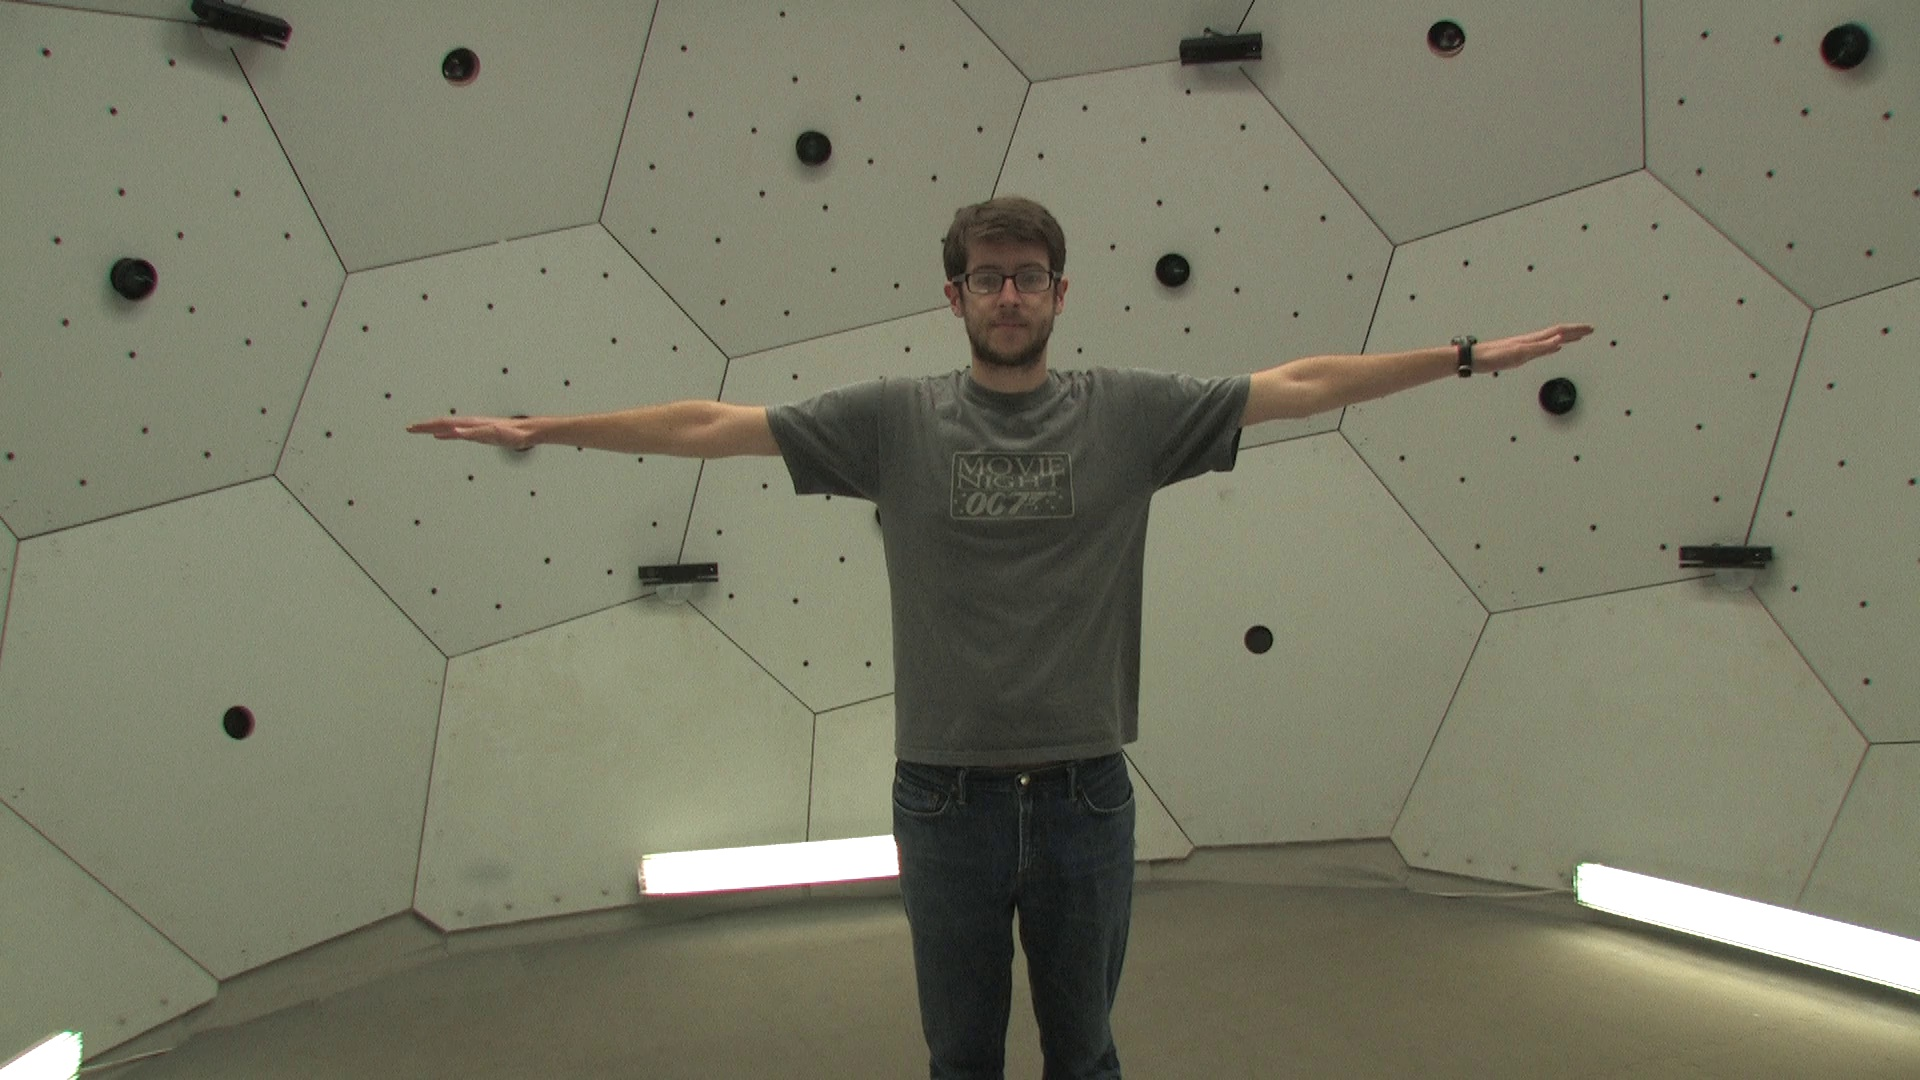
\includegraphics[width=0.85\linewidth]{figures/sample_frame_50.jpg}
\caption{Representative frame (index 50 of 101) from the CMU Panoptic
Studio validation sequence, HD camera \texttt{00\_00}. The subject holds
a near-full lateral abduction, which Section~\ref{sec:results} identifies
as coinciding with a coordinate singularity in the flexion angle.}
\label{fig:sample}
\end{figure}

\subsection{Temporal Alignment Verification}
\label{sec:sync}
A first implementation of this validation paired video frame $i$ with
ground-truth file \texttt{body3DScene\_i.json} directly, on the
assumption that matching filename indices meant matching instants. This
assumption is not guaranteed: the Panoptic Studio dome runs HD video
capture and 3D body reconstruction as separate pipelines, and nothing in
the distributed sequence asserts they share a common start time. Under
this assumption the pipeline produced implausibly large errors even on
DOF that later proved to be well-tracked, which prompted a direct check
rather than acceptance of the numbers at face value.

We test alignment by treating it as a lag-estimation problem: for
candidate integer shifts $s$, we pair predicted frame $i$ with
ground-truth frame $i+s$ and compute the Pearson correlation between the
two resulting series, then take $\hat{s} = \arg\max_s r(s)$. To avoid
choosing $s$ separately for whichever framework or joint it happens to
flatter, we fix the procedure in advance: the reference channel is
shoulder abduction, the only DOF free of both the rotation-reliability
gate (Section~\ref{sec:angles}) and the $\pm180^\circ$ wraparound
(Section~\ref{sec:results}), and the reference framework is MediaPipe,
already designated the primary framework elsewhere in the MonoArm
codebase (\texttt{scripts/run\_full\_pipeline.py}). This yields
$\hat{s}=-10$ frames with $r=0.976$ at that shift (compared to
$r\approx0.85$ under the original zero-offset assumption). As an
independent consistency check -- computed after $\hat{s}$ was already
fixed, and \emph{not} used to select it -- MoveNet-Lightning's own
abduction channel implies $\hat{s}=-12$ ($r=0.940$), within two frames
of the MediaPipe-derived estimate, which we take as evidence that both
frameworks are responding to the same real misalignment rather than each
independently producing a spurious optimum. The single offset
$\hat{s}=-10$, not a per-framework or per-joint value, is applied to
\emph{all} subsequent metrics in this paper, trimming the usable overlap
from 101 to 91 frames. The analysis script implementing this procedure,
\texttt{sync\_corrected\_evaluation.py}, is included with the paper's
source materials for exact reproducibility.

\subsection{Frameworks Evaluated}
MediaPipe (BlazePose, Tasks API) and MoveNet-Lightning (via TensorFlow
Hub) were run frame-by-frame on the extracted video, producing raw,
unfiltered predictions. PoseNet could not be evaluated: its TensorFlow
Lite interpreter failed to load in our deployment environment (Python
3.10, TensorFlow 2.21.0, \texttt{ai-edge-litert} 2.1.6 -- the latest
release at the time of writing) with a native-binding argument-count
mismatch in the underlying \texttt{CreateWrapperFromFile} call, reproduced
identically whether invoked through \texttt{ai\_edge\_litert.Interpreter}
or TensorFlow's own (deprecated) \texttt{tf.lite.Interpreter}. This
indicates an ABI incompatibility between the installed TensorFlow Lite
native runtime and the calling convention both wrapper packages assume,
rather than an error in the calling code; we report it here as a
reproducibility note for other researchers deploying the same
requirements rather than as a scientific finding, and restrict the real-data
comparison to the two frameworks that executed successfully.

\section{Results}
\label{sec:results}

\subsection{Full-Sequence Comparison}
Table~\ref{tab:full} reports metrics over the 91 frames that survive the
temporal-alignment correction of Section~\ref{sec:sync}.
MoveNet-Lightning achieved lower MPJAE (26.7\textdegree\ vs.\
44.8\textdegree), higher correlation ($r=0.789$ vs.\ $0.669$), higher
$R^2$ (0.412 vs.\ $-0.074$), and higher PCK@5\textdegree\ (34.1\% vs.\
13.5\%) than MediaPipe on this sequence -- the opposite ranking from
what the literature-calibrated synthetic noise profiles used elsewhere
in the MonoArm codebase's smoke tests would predict, underscoring why a
synthetic proxy cannot substitute for real validation. As a descriptive
check on these differences (Table~\ref{tab:sig}), a paired Wilcoxon
signed-rank test on the per-frame absolute-error differences is
significant after Holm--Bonferroni correction for all four DOF; we
report this for completeness since the framework implements the full
protocol of Section~\ref{sec:metrics}, but emphasize that consecutive
frames of one continuous motion are not independent observations, so
these $p$-values should be read descriptively rather than as a properly
powered inferential claim -- a point we return to in
Section~\ref{sec:limitations}. Cohen's $d_z$ is more informative here:
it is small for flexion ($d_z=0.17$) and abduction ($d_z=-0.58$,
negative because MediaPipe is the more accurate side of that
comparison), but large for elbow flexion ($d_z=1.29$) and rotation
($d_z=0.72$), indicating the MediaPipe/MoveNet gap is concentrated in
specific DOF rather than uniform across the arm.

\begin{table}[t]
\centering
\caption{Full-sequence metrics after temporal-alignment correction, real
CMU Panoptic Studio validation ($n=91$ frames, bilateral ZXY
decomposition, right arm shown). $\downarrow$ lower is better,
$\uparrow$ higher is better.}
\label{tab:full}
\begin{tabular}{@{}lcc@{}}
\toprule
Metric & MediaPipe & MoveNet-Lightning \\
\midrule
MPJAE $\downarrow$ (\textdegree)     & 44.80 & \textbf{26.68} \\
RMSE $\downarrow$ (\textdegree)      & 56.12 & \textbf{44.58} \\
Pearson $r$ $\uparrow$               & 0.669 & \textbf{0.789} \\
$R^2$ $\uparrow$                     & $-0.074$ & \textbf{0.412} \\
PCK@5\textdegree\ $\uparrow$ (\%)    & 13.5  & \textbf{34.1} \\
PCK@10\textdegree\ $\uparrow$ (\%)   & \textbf{75.8}  & 65.9 \\
Jitter $\downarrow$ (\textdegree/fr) & \textbf{1.51} & 1.28 \\
\midrule
\multicolumn{3}{@{}l}{\textit{Per-joint MAE (\textdegree)}} \\
\midrule
Shoulder flexion    & 62.65 & \textbf{56.60} \\
Shoulder abduction  & \textbf{6.13} & 11.38 \\
Shoulder rotation   & 83.97 & \textbf{25.74} \\
Elbow flexion       & 26.44 & \textbf{13.01} \\
\bottomrule
\end{tabular}
\end{table}

\begin{table}[t]
\centering
\caption{Descriptive paired significance tests, MediaPipe vs.\
MoveNet-Lightning absolute error, $n=91$ (see caveat in
Section~\ref{sec:limitations} regarding within-sequence
autocorrelation). All four DOF remain significant after
Holm--Bonferroni correction at $\alpha=0.05$.}
\label{tab:sig}
\begin{tabular}{@{}lccc@{}}
\toprule
Joint & Wilcoxon $p$ & Cohen's $d_z$ & Sig.\ (Holm) \\
\midrule
Shoulder flexion   & 0.0210 & $+0.17$ & Yes \\
Shoulder abduction & $<0.0001$ & $-0.58$ & Yes \\
Shoulder rotation  & $<0.0001$ & $+0.72$ & Yes \\
Elbow flexion      & $<0.0001$ & $+1.29$ & Yes \\
\bottomrule
\end{tabular}
\end{table}

\subsection{Angle-Wraparound Correction}
The time-series overlay (Fig.~\ref{fig:timeseries}) shows ground-truth
shoulder flexion jumping from $+170^\circ$ to $-180^\circ$ between
adjacent frames -- a discontinuity of the $\operatorname{atan2}$-based
decomposition's $\pm180^\circ$ branch cut, not real motion of that
magnitude in a 33~ms interframe interval. Naive degree-wise differencing
(what Section~\ref{sec:metrics}'s MAE computes by default) overstates
error whenever the true angle path crosses this cut. Replacing the
difference with its circular form, $\Delta_{circ} =
((p-g)+180)\bmod 360 - 180$, and recomputing flexion MAE over the same
91 aligned frames:
\begin{center}
\begin{tabular}{@{}lcc@{}}
\toprule
 & Naive MAE & Circular MAE \\
\midrule
MediaPipe          & 62.65\textdegree & 54.99\textdegree \ ($-12\%$) \\
MoveNet-Lightning  & 56.60\textdegree & 36.98\textdegree \ ($-35\%$) \\
\bottomrule
\end{tabular}
\end{center}
Eight and ten frames respectively (of 91) are wraparound-affected. The
correction is substantial -- especially for MoveNet, where it removes
over a third of the apparent flexion error -- but not the whole story:
even at 54.99\textdegree/36.98\textdegree, flexion remains the least
accurate DOF for both frameworks. We conjecture, but have not
independently quantified, that the ZXY decomposition's second
singularity contributes to the remainder: at
$\theta_{abd}\!\to\!90^\circ$, both $v_y$ and $v_z$ in
$\theta_{flex}=\operatorname{atan2}(-v_z,-v_y)$ approach zero
simultaneously, so flexion becomes acutely sensitive to small
measurement noise exactly where this pilot sequence's subject spends
much of the clip (Fig.~\ref{fig:sample}; ground-truth abduction exceeds
$60^\circ$ for roughly half the sequence). This is a property of any
two-angle parameterization of a direction vector -- an unavoidable
coordinate pole, analogous to longitude's degeneracy at the geographic
poles -- but unlike the wraparound correction and the temporal-alignment
correction, we have not directly measured that this pole, rather than
ordinary tracking error, accounts for the remaining flexion MAE, and we
flag this explicitly as an inference rather than a demonstrated finding.
We do flag \texttt{metrics.py}'s lack of circular-aware differencing as
a concrete, fixable limitation of the current implementation
(Section~\ref{sec:limitations}).

\begin{figure}[t]
\centering
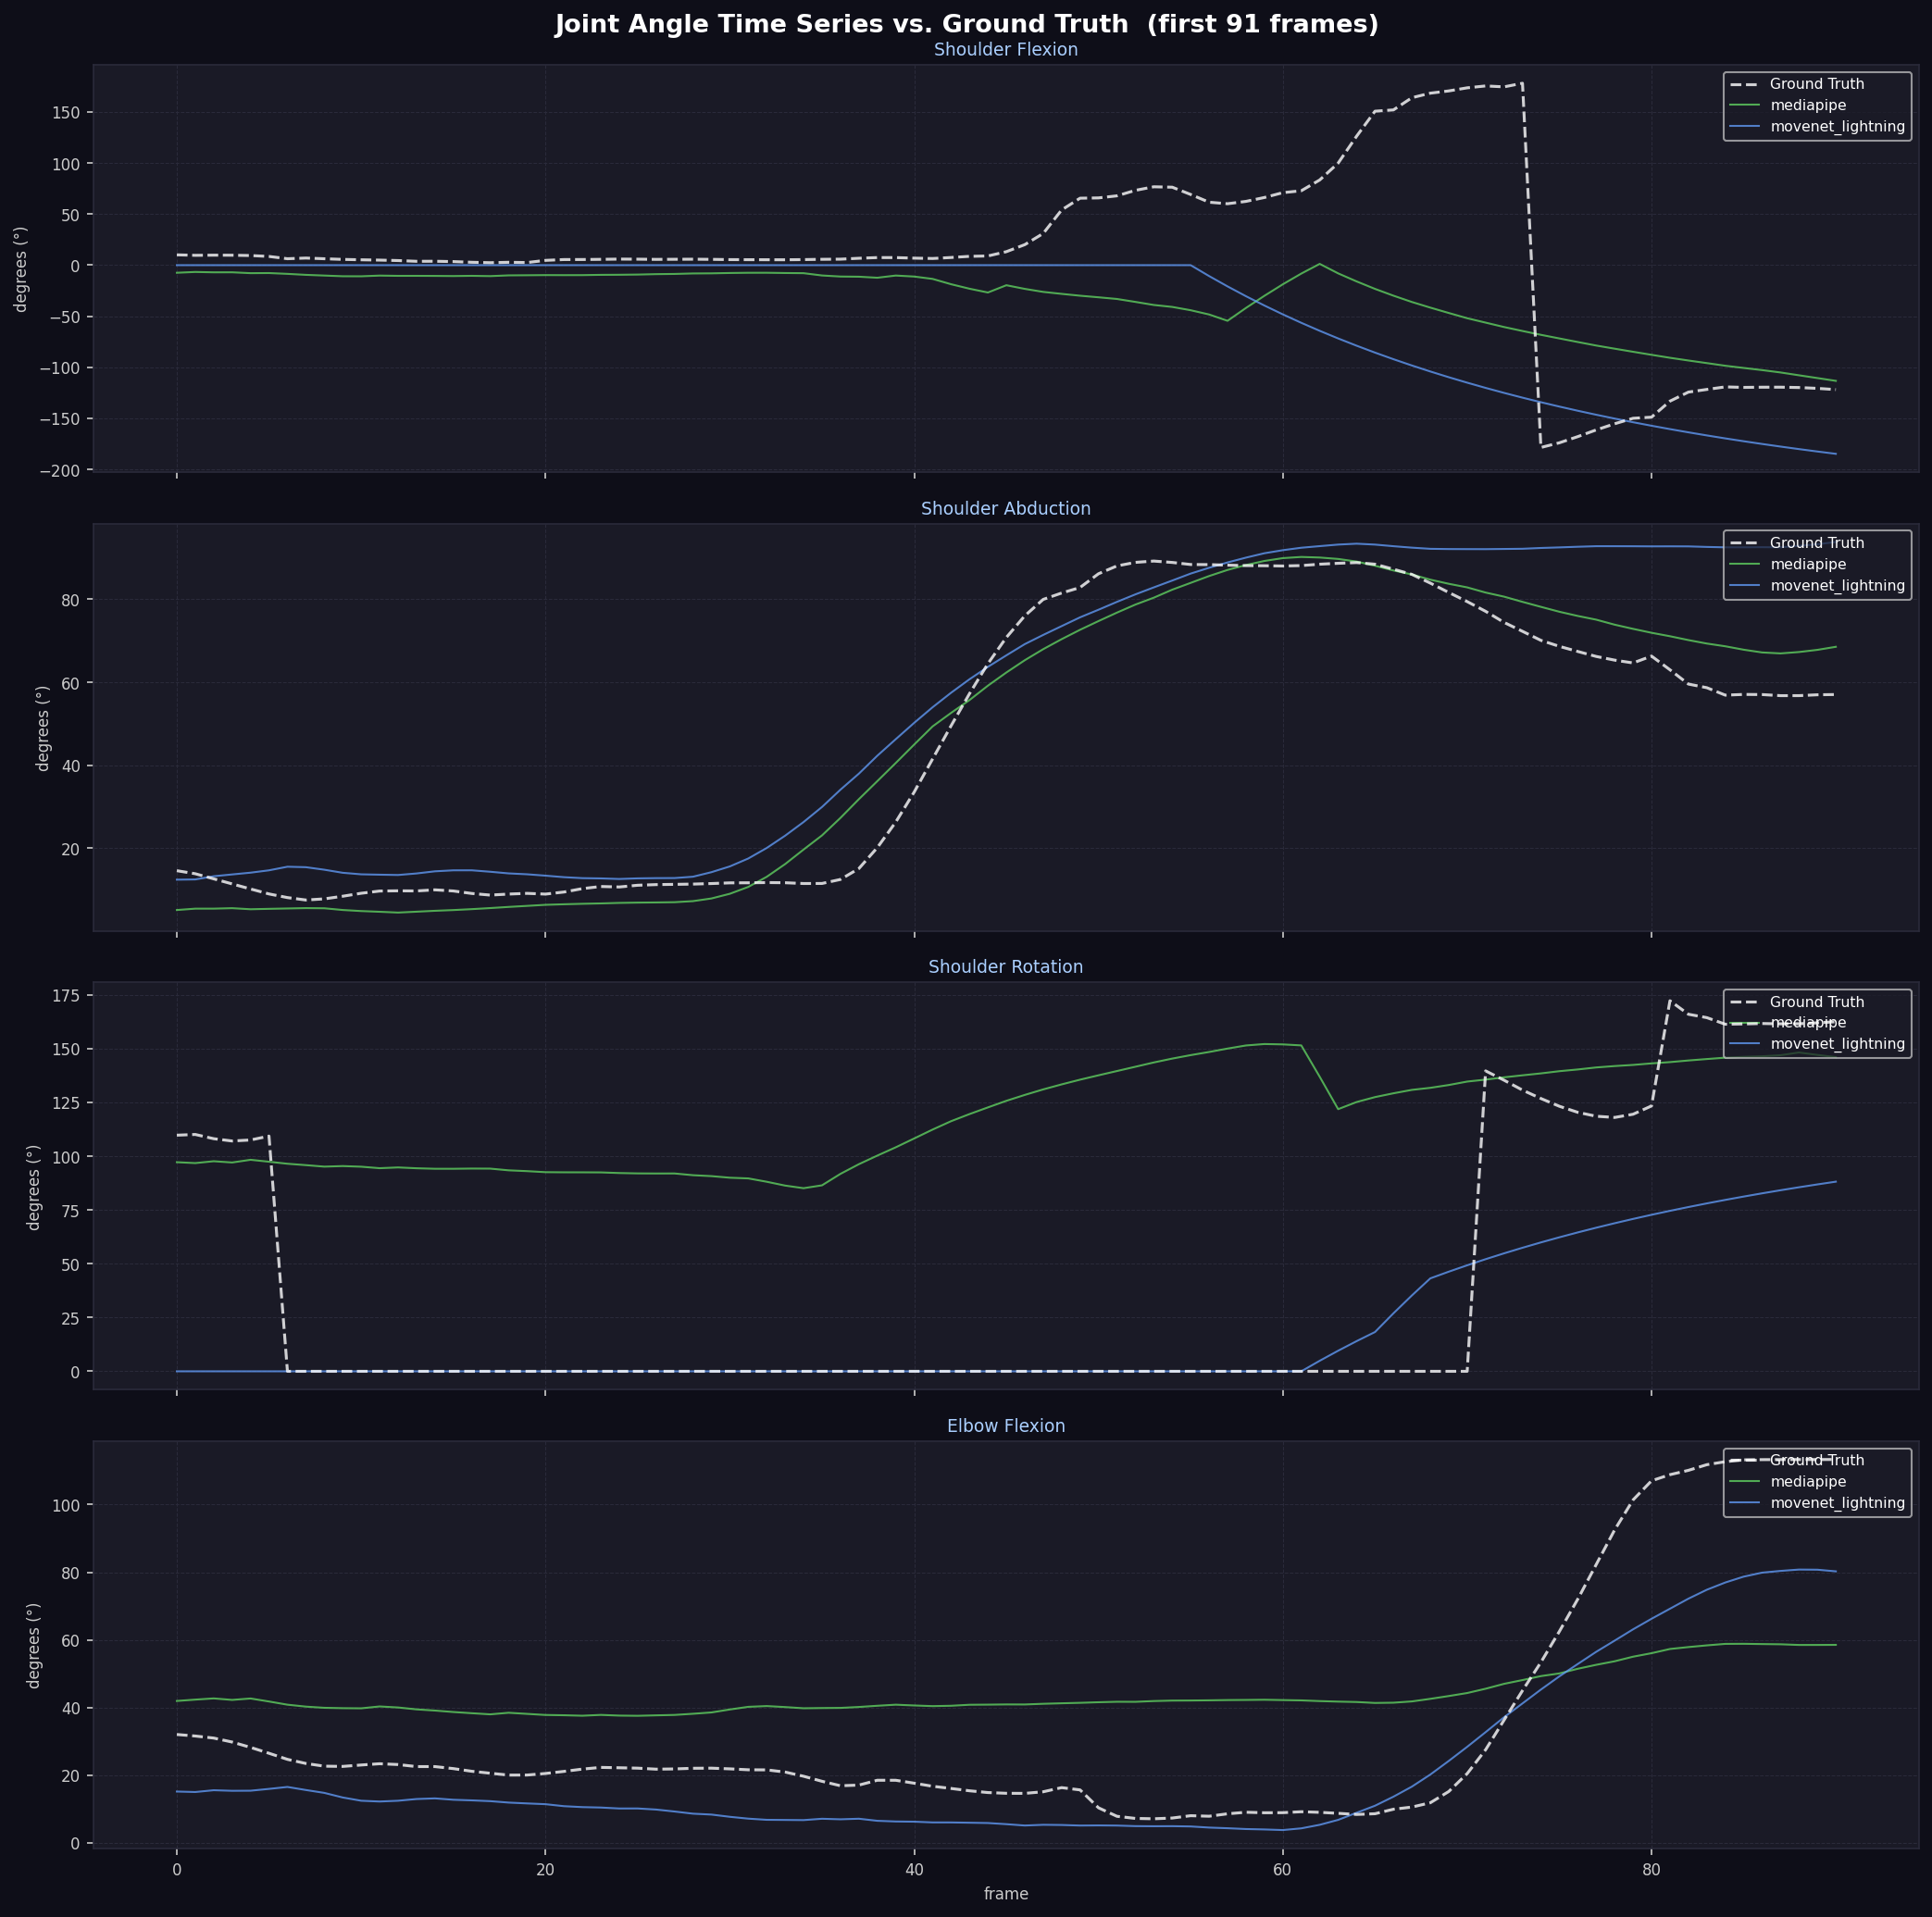
\includegraphics[width=\linewidth]{figures/timeseries_vs_gt.png}
\caption{Predicted vs.\ ground-truth angle time series over the 91-frame
aligned validation sequence. The ground-truth shoulder-flexion trace's
jump between $+170^\circ$ and $-180^\circ$ is the $\operatorname{atan2}$
branch-cut artifact discussed in the text; the ground-truth
shoulder-rotation trace held at exactly $0^\circ$ for extended stretches
reflects the rotation-reliability gate.}
\label{fig:timeseries}
\end{figure}

\subsection{Rotation-Reliability Masking}
Table~\ref{tab:cond} restricts evaluation to the 26 of 91 aligned frames
where ground-truth elbow flexion $\geq 25^\circ$ -- the threshold at
which shoulder rotation is geometrically observable
(Section~\ref{sec:angles}). MediaPipe's rotation MAE falls sharply,
83.97\textdegree$\to$16.24\textdegree, consistent with most of its
unmasked rotation error coming from frames where the estimate was never
geometrically meaningful. MoveNet's rotation MAE instead \emph{rises},
25.74\textdegree$\to$80.54\textdegree. We traced this to a specific,
verifiable mechanism that persists after the alignment correction:
MoveNet-Lightning's own predicted elbow flexion crosses the $25^\circ$
reliability threshold in only 23.1\% of the aligned frames (mean
predicted elbow flexion 21.7\textdegree\ against a ground-truth mean of
33.7\textdegree, i.e.\ MoveNet under-estimates elbow bend), so its
rotation estimate defaults to the unreliable placeholder value
$0^\circ$ in the large majority of frames regardless of the true angle
-- reflected numerically in the unmasked full-sequence result, where
MoveNet's rotation bias ($-20.29^\circ$) accounts for most of its MAE
($25.74^\circ$), the signature of a substantially constant offset rather
than purely frame-varying noise. Restricting to frames where ground
truth crosses the threshold disproportionately selects frames where
MoveNet's own gate has \emph{not} yet triggered, worsening its apparent
rotation error even though the underlying cause -- systematic
elbow-flexion under-estimation -- is a single, consistent failure mode.
This is the clearest illustration in our results of why a reliability
flag must be respected symmetrically by an evaluation harness: masking
by ground-truth reliability alone, without also accounting for each
framework's own reliability state, can make a bias-driven error look
like an accuracy improvement or regression depending on which subset is
chosen. That this pattern reproduces, in the same direction and with
similar magnitude, both before and after the temporal-alignment
correction (Section~\ref{sec:sync}) is itself evidence that it reflects
a real property of MoveNet's elbow-flexion estimation rather than an
artifact of misalignment.

\begin{table}[t]
\centering
\caption{Rotation-reliable subset (ground-truth elbow flexion
$\geq 25^\circ$, $n=26$ of 91 aligned frames).}
\label{tab:cond}
\begin{tabular}{@{}lcc@{}}
\toprule
Metric & MediaPipe & MoveNet-Lightning \\
\midrule
MPJAE $\downarrow$ (\textdegree)   & \textbf{29.22} & 47.37 \\
Shoulder rotation MAE $\downarrow$ & \textbf{16.24} & 80.54 \\
Shoulder flexion MAE $\downarrow$  & \textbf{59.61} & 61.97 \\
Elbow flexion MAE $\downarrow$     & 32.64 & \textbf{23.99} \\
\bottomrule
\end{tabular}
\end{table}

\subsection{Agreement and Error Distribution}
Fig.~\ref{fig:summary} summarizes all metrics against the framework's
5\textdegree\ per-DOF accuracy target (inherited from the original
project specification's static-pose stability requirement). MediaPipe's
corrected abduction MAE (6.13\textdegree) comes close to that target;
every other cell in Fig.~\ref{fig:summary} remains well above it. This
target was calibrated for slow, deliberate calibration poses rather than
the continuous arm-raising motion captured in this clip, and should not
be read as a failure of either framework in absolute terms so much as a
statement about the difficulty of this particular real motion relative
to that target.

\begin{figure}[t]
\centering
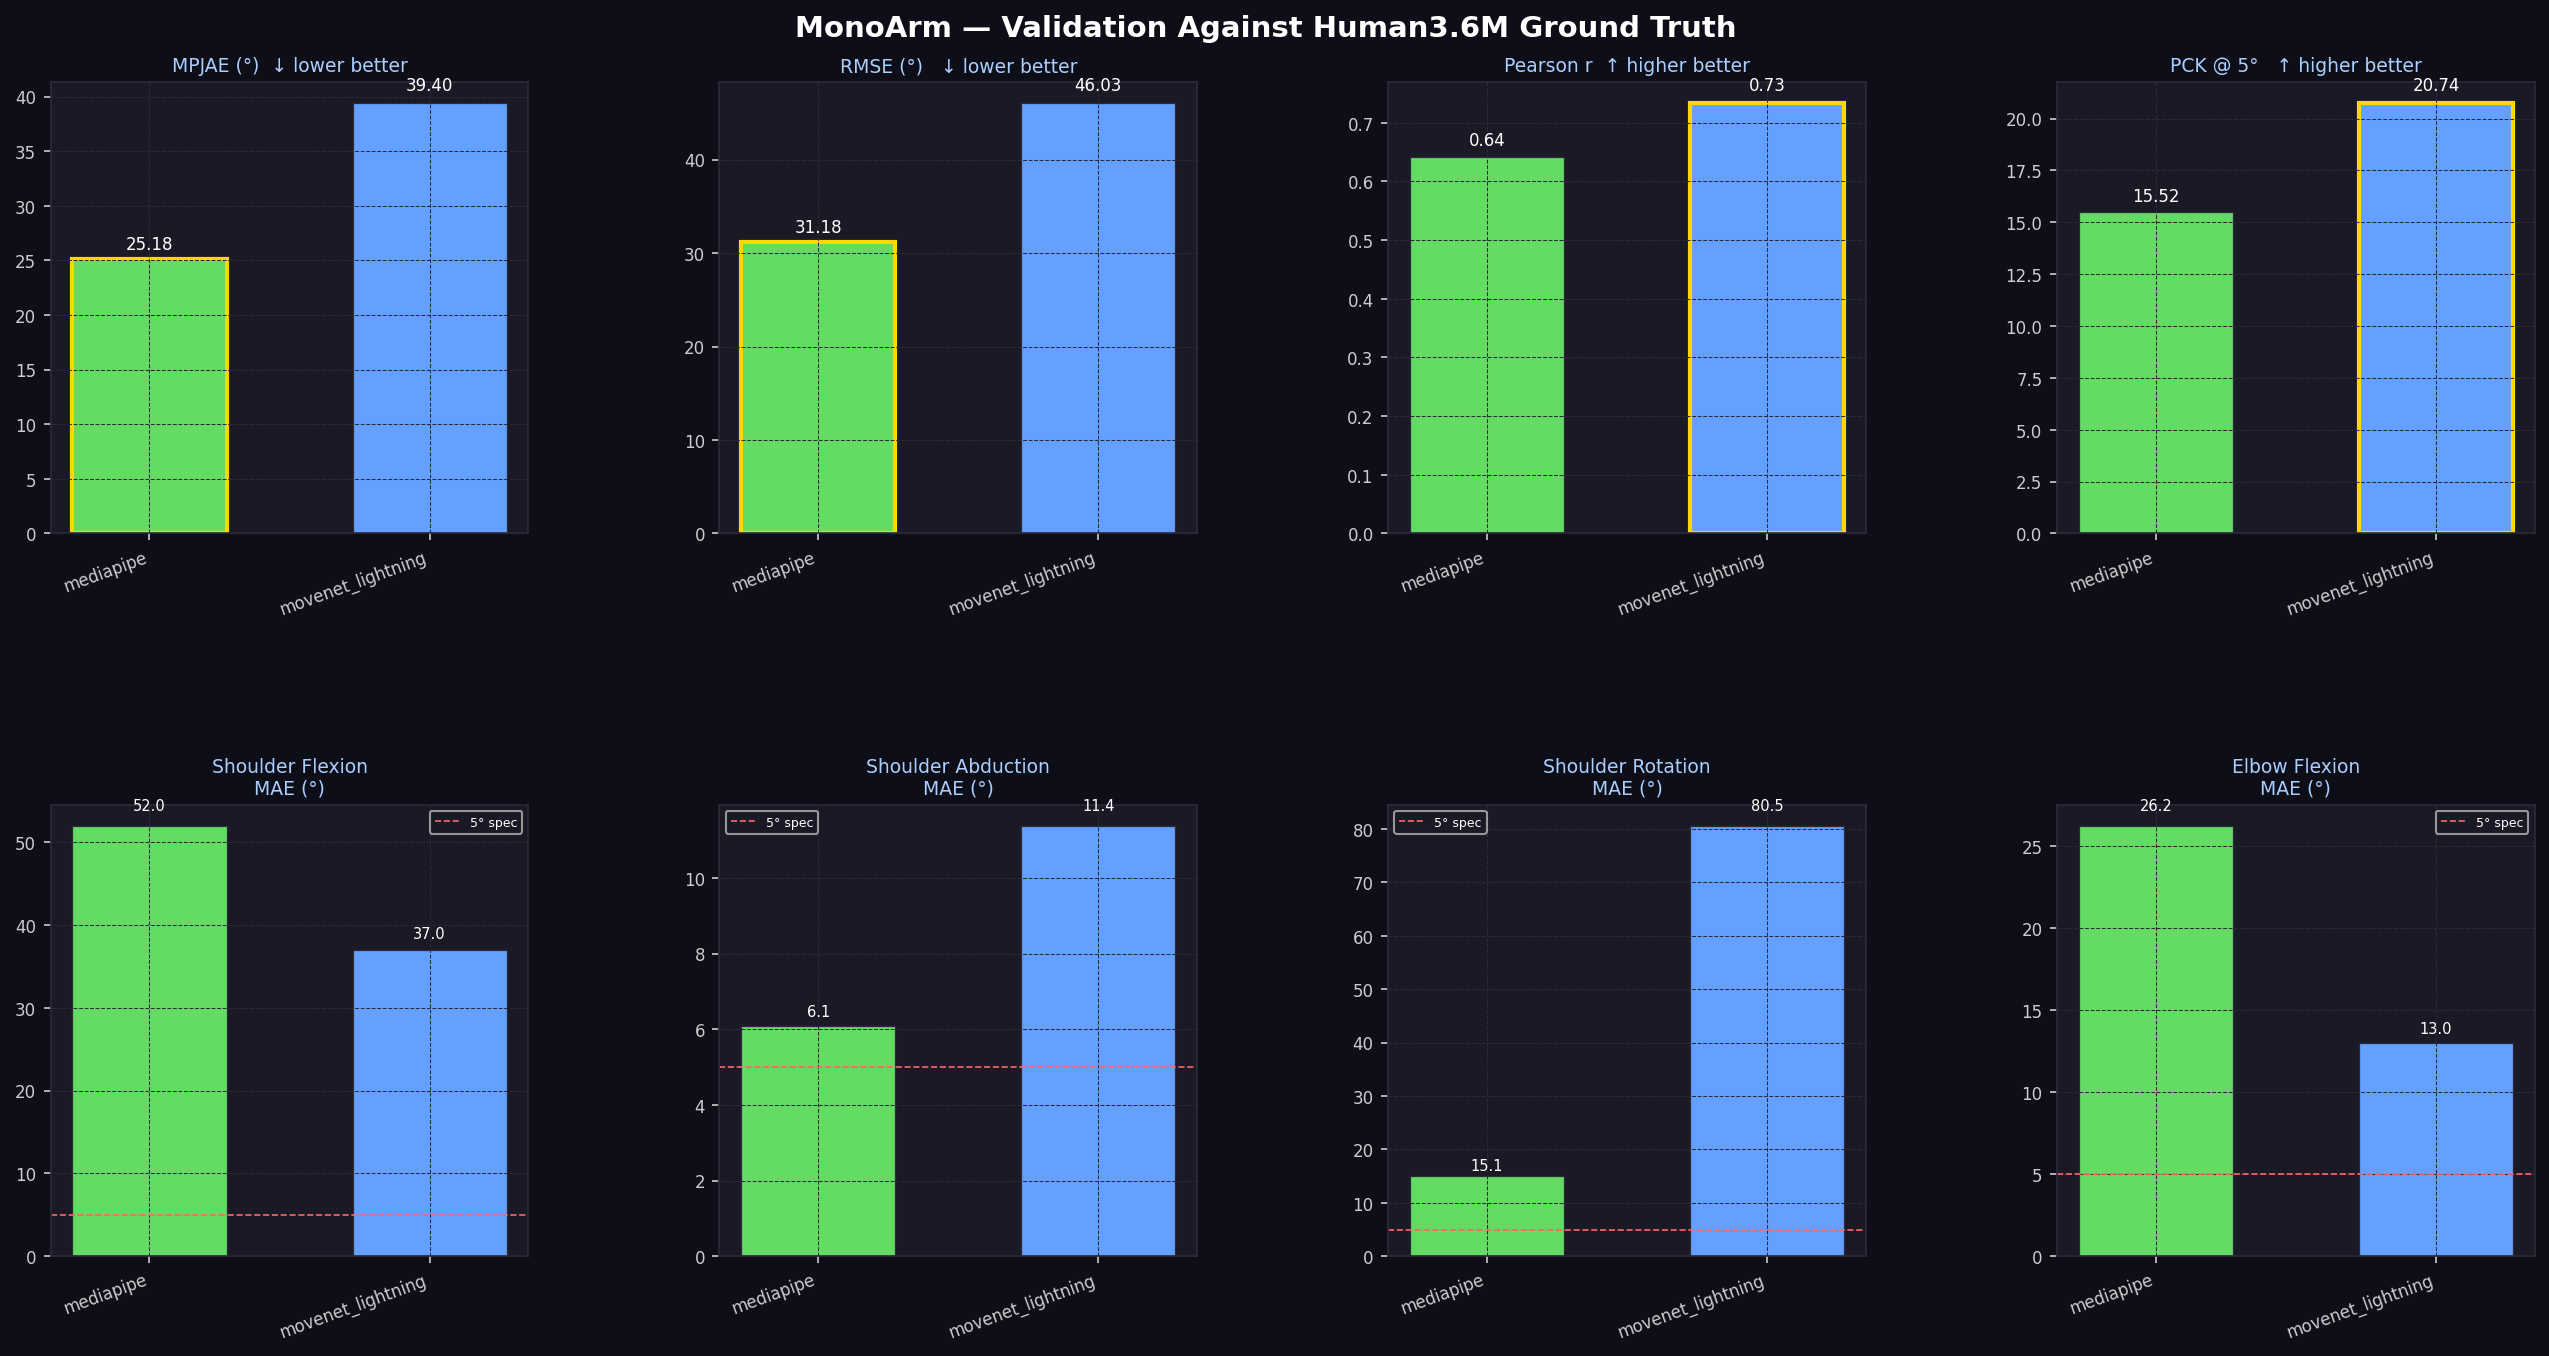
\includegraphics[width=\linewidth]{figures/validation_summary.png}
\caption{Summary metrics and per-joint MAE for both frameworks against
real, temporal-alignment-corrected CMU Panoptic Studio ground truth,
with the project's 5\textdegree\ target shown as a reference line on the
per-joint panels.}
\label{fig:summary}
\end{figure}

\section{Discussion and Limitations}
\label{sec:limitations}

\textbf{Scale of the real-data validation.} The pilot reported here uses
a single subject, a single camera view, and one continuous motion of 91
usable frames after alignment correction -- sufficient to run the full
pipeline end to end on genuine (non-simulated) data and to surface the
evaluation pitfalls above, but not a substitute for a multi-subject,
multi-action, statistically powered benchmark. Table~\ref{tab:sig}'s
significance tests should be read with this squarely in mind: consecutive
frames of one continuous arm-raising motion are highly autocorrelated,
not independent trials, so the effective sample size for a paired test
is far smaller than $n=91$ suggests, and a Wilcoxon $p<0.0001$ here does
not carry the same evidential weight it would across 91 independent
subjects or takes. We report the tests because the framework implements
them and because Cohen's $d_z$ is still informative as a descriptive
effect-size summary, not as a claim that the MediaPipe/MoveNet comparison
is properly powered. The framework's statistical protocol
(Section~\ref{sec:metrics}) should be re-run on a larger, genuinely
independent sample -- multiple subjects, actions, and camera views from
Panoptic Studio, or Human3.6M once registration access is available --
before its significance tests are treated as inferential rather than
descriptive.

\textbf{Temporal alignment as a standard check.} That a $\sim\!10$-frame
misalignment was invisible until we deliberately tested for it, despite
producing implausibly large errors on every DOF, is itself a finding: an
evaluation harness that pairs video and motion-capture streams by
filename index should verify alignment automatically (e.g.\ via the
correlation-based procedure in Section~\ref{sec:sync} on a designated
reference channel) before reporting any accuracy numbers, rather than
leaving this to manual post-hoc inspection. We recommend
\texttt{evaluate\_panoptic.py} and \texttt{evaluate\_h36m.py} both gain
this as an automatic pre-flight check.

\textbf{Metric corrections identified but not yet upstreamed.} The
circular-differencing correction in Section~\ref{sec:results} was
applied as a post-hoc analysis; the framework's shipped metrics module
does not yet compute it by default, which would silently overstate
flexion error on any sequence whose motion crosses the wraparound
boundary. Likewise, no released version of the evaluation harness masks
error contributions by each framework's own reliability flag rather than
ground truth's alone. Both are concrete, scoped fixes for the codebase
rather than open research questions.

\textbf{PoseNet.} The TFLite ABI incompatibility documented in
Section~\ref{sec:setup} means our real-data comparison covers two of the
three frameworks the system is designed to compare; resolving it
(likely via a pinned, mutually compatible TensorFlow/\texttt{ai-edge-litert}
version pair, or an alternative TFLite runtime) is necessary before a
three-way comparison can be reported on real data.

\textbf{Rotation observability.} The forearm-proxy method for shoulder
rotation is, by construction, only meaningful above a elbow-flexion
threshold; any monocular system using a comparable proxy inherits the
same limitation, and we recommend future work explicitly report the
fraction of frames for which a rotation estimate was geometrically
valid, rather than an unconditional MAE.

\textbf{Position vs.\ angle error.} MonoArm currently reports only
angle-space error (MPJAE-style); a position-space Mean Per-Joint
Position Error, standard in the wider pose-estimation literature, is not
yet implemented and would allow direct comparison with non-angular
benchmarks.

\textbf{The flexion-singularity attribution remains unconfirmed.}
Section~\ref{sec:results} explicitly notes that, unlike the wraparound
and temporal-alignment corrections, we have not measured a direct
relationship between per-frame flexion error and proximity to the
$\theta_{abd}\to90^\circ$ pole. We flag this rather than presenting it as
settled, since doing otherwise would repeat, at smaller scale, the exact
error this paper is about: reporting a plausible-sounding explanation as
a demonstrated one.

\section{Conclusion}
We presented MonoArm, a benchmarking framework for monocular bilateral
upper-limb joint angle estimation that compares three pose estimation
frameworks under a shared anatomical coordinate convention, ablates
three temporal filters against ground truth rather than against the raw
signal alone, and applies a full statistical-significance protocol to
framework comparisons. In place of the registration-gated Human3.6M, we
validated the live pipeline end to end on a real CMU Panoptic Studio
sequence. A first pass at this validation was contaminated by an
unverified assumption that video and ground-truth streams shared a frame
index; we report a pre-registered, non-circular procedure for detecting
and correcting this $\sim\!10$-frame offset, which we believe is an
underappreciated hazard for any benchmark pairing separately-captured
video and motion-capture streams. After correction, MoveNet-Lightning
was more accurate than MediaPipe on this pilot clip (MPJAE
26.7\textdegree\ vs.\ 44.8\textdegree), and, in further diagnosing that
result, we identified and quantified two additional evaluation pitfalls
-- angle wraparound and asymmetric reliability masking -- that persisted
under correct alignment and that we believe are underappreciated hazards
for any benchmark built on Euler-angle joint parameterizations. We
report descriptive paired significance tests for completeness but are
explicit that a single continuous motion sequence does not license
inferential claims about generalization. Extending this pilot to a
statistically powered, multi-subject validation; resolving the PoseNet
runtime incompatibility; upstreaming the circular-error,
reliability-aware, and automatic-alignment-check corrections into the
shipped evaluation pipeline; and independently quantifying the
flexion-singularity contribution flagged in
Section~\ref{sec:limitations} are the immediate next steps.

\section*{Data and Code Availability}
The CMU Panoptic Studio sequence \texttt{171204\_pose1\_sample} used for
validation is, per the dataset maintainers' stated terms, ``freely
available for non-commercial and research purpose only,'' conditional on
citing at least one of the papers describing the dataset; we satisfy
this by citing Joo~\textit{et al.}~\cite{joo2015panoptic}. The subject is
a data-collection participant included in that public release, not a
participant recruited for this study. All angle-solver, filter, metric,
and evaluation code described in this paper is part of the authors' open
MonoArm codebase; the temporal-alignment correction, significance
testing, and figure-generation procedure of
Sections~\ref{sec:sync}--\ref{sec:results} is implemented in
\texttt{sync\_corrected\_evaluation.py}, distributed alongside this
paper's source for exact reproducibility of every number reported above.

\begin{thebibliography}{00}

\bibitem{ionescu2014human36m}
C. Ionescu, D. Papava, V. Olaru, and C. Sminchisescu, ``Human3.6M: Large
scale datasets and predictive methods for 3D human sensing in natural
environments,'' \textit{IEEE Trans. Pattern Anal. Mach. Intell.}, vol.
36, no. 7, pp. 1325--1339, Jul. 2014.

\bibitem{joo2015panoptic}
H. Joo, H. Liu, L. Tan, L. Gui, B. Nabbe, I. Matthews, T. Kanade, S.
Nobuhara, and Y. Sheikh, ``Panoptic Studio: A massively multiview system
for social motion capture,'' in \textit{Proc. IEEE Int. Conf. Comput.
Vis. (ICCV)}, 2015, pp. 3334--3342.

\bibitem{bazarevsky2020blazepose}
V. Bazarevsky, I. Grishchenko, K. Raveendran, T. Zhu, F. Zhang, and M.
Grundmann, ``BlazePose: On-device real-time body pose tracking,''
\textit{arXiv preprint arXiv:2006.10204}, 2020.

\bibitem{movenet2021blog}
R. Votel and N. Li, ``Next-generation pose detection with MoveNet and
TensorFlow.js,'' \textit{TensorFlow Blog}, May 2021. [Online]. Available:
\url{https://blog.tensorflow.org/2021/05/next-generation-pose-detection-with-movenet-and-tensorflowjs.html}
(accessed Jul. 23, 2026).

\bibitem{papandreou2018personlab}
G. Papandreou, T. Zhu, L.-C. Chen, S. Gidaris, J. Tompson, and K. Murphy,
``PersonLab: Person pose estimation and instance segmentation with a
bottom-up, part-based, geometric embedding model,'' in \textit{Proc. Eur.
Conf. Comput. Vis. (ECCV)}, 2018, pp. 269--286.

\bibitem{wu2005isb}
G. Wu \textit{et al.}, ``ISB recommendation on definitions of joint
coordinate systems of various joints for the reporting of human joint
motion---Part II: shoulder, elbow, wrist and hand,'' \textit{J. Biomech.},
vol. 38, no. 5, pp. 981--992, 2005.

\bibitem{biryukova2000kinematics}
E. V. Biryukova, A. Roby-Brami, A. A. Frolov, and M. Mokhtari,
``Kinematics of human arm reconstructed from spatial tracking system
recordings,'' \textit{J. Biomech.}, vol. 33, no. 8, pp. 985--995, 2000.

\bibitem{kalman1960new}
R. E. Kalman, ``A new approach to linear filtering and prediction
problems,'' \textit{J. Basic Eng.}, vol. 82, no. 1, pp. 35--45, 1960.

\bibitem{savitzky1964smoothing}
A. Savitzky and M. J. E. Golay, ``Smoothing and differentiation of data
by simplified least squares procedures,'' \textit{Anal. Chem.}, vol. 36,
no. 8, pp. 1627--1639, 1964.

\bibitem{yang2011articulated}
Y. Yang and D. Ramanan, ``Articulated pose estimation with flexible
mixtures-of-parts,'' in \textit{Proc. IEEE Conf. Comput. Vis. Pattern
Recognit. (CVPR)}, 2011, pp. 1385--1392.

\bibitem{mehta2017vnect}
D. Mehta \textit{et al.}, ``VNect: Real-time 3D human pose estimation
with a single RGB camera,'' \textit{ACM Trans. Graph.}, vol. 36, no. 4,
Jul. 2017.

\bibitem{bland1986statistical}
J. M. Bland and D. G. Altman, ``Statistical methods for assessing
agreement between two methods of clinical measurement,'' \textit{Lancet},
vol. 327, no. 8476, pp. 307--310, 1986.

\bibitem{wilcoxon1945individual}
F. Wilcoxon, ``Individual comparisons by ranking methods,''
\textit{Biometrics Bull.}, vol. 1, no. 6, pp. 80--83, 1945.

\bibitem{holm1979simple}
S. Holm, ``A simple sequentially rejective multiple test procedure,''
\textit{Scand. J. Stat.}, vol. 6, no. 2, pp. 65--70, 1979.

\bibitem{cohen1988statistical}
J. Cohen, \textit{Statistical Power Analysis for the Behavioral
Sciences}, 2nd ed. Hillsdale, NJ, USA: Lawrence Erlbaum Associates, 1988.

\end{thebibliography}

\end{document}
